%%%%%%%%%%%%%%%%%%%%%%%%%%%%%%%%%%%%%%%%%
% CSE 4316/4317 Sprint Report Template
% Version 1.0 (2/18/2018)
% Author: Christopher D. McMurrough
%%%%%%%%%%%%%%%%%%%%%%%%%%%%%%%%%%%%%%%%%

%----------------------------------------------------------------------------------------
%	PACKAGES AND DOCUMENT CONFIGURATIONS
%----------------------------------------------------------------------------------------

\documentclass{article}
\usepackage{siunitx}
\usepackage{graphicx}
\usepackage{amsmath}
\setlength\parindent{0pt}

\usepackage[letterpaper, portrait, margin=1in]{geometry}

%----------------------------------------------------------------------------------------
%	DOCUMENT SECTIONS
%----------------------------------------------------------------------------------------

% report title
\title{Sprint 3 Report \\ CSE 4316}

% author name
\author{Atafo Abure}

% date of assignment submission
\date{November 14, 2019}

\begin{document}
\maketitle
\begin{center}
\begin{tabular}{l r}

% sprint start date
Sprint start date: & October 24th, 2019 \\

% sprint end date
Sprint end date: & November 14th, 2019 \\

% project title
Project title: & Smart Shutters \\

% team name
Team name: & No SHUT Eye \\

% team members
Partners: 	& Haris Qureshi\\
			& David Nquyen\\
			& Deion Nwaefulu \\
        	& Aditya Rajguru \\
Instructor: & Shawn Gieser
\end{tabular}
\end{center}

% sprint goal
\section{Sprint Goal}
Finish Architectural Design Specificiation Document \\
Establish Framework for WiFi Communication \\
Establish Framework for Bluetooth Communication \\

% sprint backlog
\section{Sprint Backlog}
Breakdown of planned tasks assigned to team (work units expressed in days) \\ % work units do not have to be hours, change text accordingly

% ADD OR REMOVE ROWS FROM THE TABLE AS NECESSARY (DO NOT LEAVE BLANK ROWS!)
\begin{tabular}{| p{4in} | >{\centering\arraybackslash} p{1in} | >{\centering\arraybackslash} p{1in} |}
\hline
TASK DESCRIPTION & ESTIMATED WORK & ACTUAL WORK \\ \hline
Process Modelling & 3 & 1 \\ \hline
Finalizing Hardware Details & 5 & 1 \\ \hline
Product Conception & 1 & 1 \\ \hline
Product Description & 1 & 1 \\ \hline
Customer Requirements & 1 & 1 \\ \hline
Packaging Requirements & 1 & 1 \\ \hline
Safety Requirements & 1 & 1 \\ \hline
Performance Requirements & 1 & 1 \\ \hline
Maintenance and Support Requirements & 1 & 1 \\ \hline
\textbf{TOTAL} & \textbf{15}  & \textbf{9} \\ \hline
\end{tabular}

\pagebreak

% individual time summary
\section{Individual Time Expenditures}
Summary of tasks performed by the individual (work units expressed in days) \\ % work units do not have to be hours, change text accordingly

% ADD OR REMOVE ROWS FROM THE TABLE AS NECESSARY (DO NOT LEAVE BLANK ROWS!)
% PERCENT COMPLETE DESCRIBES THE STATE OF THE TASK AS OF THE LAST SPRINT DAY (WAS IT FINISHED? IF NOT, APPROXIMATELY HOW "COMPLETE" IS THE TASK)
\begin{tabular}{| p{4in} | >{\centering\arraybackslash} p{1in} | >{\centering\arraybackslash} p{1in} |}
\hline
TASK DESCRIPTION & ACTUAL WORK & PERCENT COMPLETE \\ \hline
Process Modelling & 1 & 100\% \\ \hline
Product Conception & 1 & 100\% \\ \hline
Product Description & 1 & 100\% \\ \hline
Customer Requirements & 1 & 100\% \\ \hline
Packaging Requirements & 1 & 100\% \\ \hline
Safety Requirements & 1 & 100\% \\ \hline
Performance Requirements & 1 & 100\% \\ \hline
\textbf{TOTAL} & \textbf{7}  & \textbf{-} \\ \hline
\end{tabular}

% burndown chart
\section{Team Burndown Chart}
Burndown chart showing day-to-day progress on sprint tasks. Ideal (baseline) daily effort and actual daily effort of the team are both shown in the figure below.
\begin{figure}[h]
\begin{center}
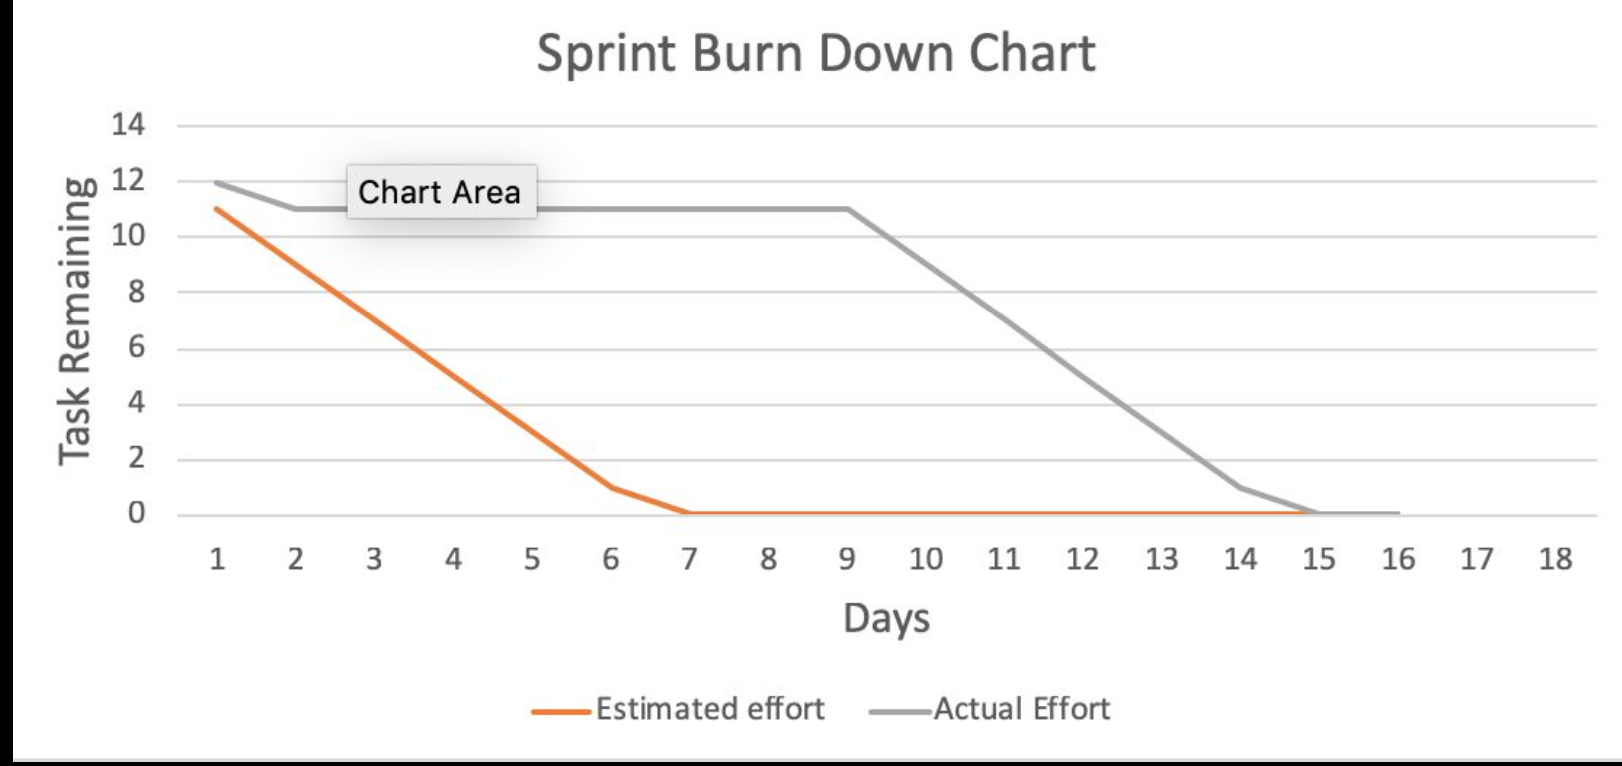
\includegraphics[width=1.0\textwidth]{Sprint2Burndown} % Include the image burndown.png
\end{center}
\end{figure}

\pagebreak

%individual sprint retrospective
\section{Individual Retrospective}
The following lists describe actions (as an individual) that will be started, stopped, or continued during the next sprint to maximize work efficiency. \\

Actions and/or items to \textbf{start} doing in the next sprint (top 3)
\begin{itemize}
\begin{item}
Start manufacturing developer Board
\end{item}
\begin{item}
Research on developer Board to use with chip
\end{item}
\begin{item}
Order and Manufacture Hardware 
\end{item}
\end{itemize}

Actions and/or items to \textbf{stop} doing in the next sprint (top 3)
\begin{itemize}
\begin{item}
SRS Document
\end{item}
\begin{item}
Process Modeling
\end{item}
\begin{item}
Gathering Requirements
\end{item}
\end{itemize}

Actions and/or items to \textbf{continue} doing in the next sprint (top 3)
\begin{itemize}
\begin{item}
Research on Bluetooth and Wi-Fi communications
\end{item}
\begin{item}
Research on motors and power consumption
\end{item}
\begin{item}
Research on chip functionality and Hardware compatibility
\end{item}
\end{itemize}

\end{document}